\documentclass[a4paper]{book}
\usepackage{makeidx}
\usepackage{graphicx}
\usepackage{multicol}
\usepackage{float}
\usepackage{listings}
\usepackage{color}
\usepackage{ifthen}
\usepackage[table]{xcolor}
\usepackage{textcomp}
\usepackage{alltt}
\usepackage{ifpdf}
\ifpdf
\usepackage[pdftex,
            pagebackref=true,
            colorlinks=true,
            linkcolor=blue,
            unicode
           ]{hyperref}
\else
\usepackage[ps2pdf,
            pagebackref=true,
            colorlinks=true,
            linkcolor=blue,
            unicode
           ]{hyperref}
\usepackage{pspicture}
\fi
\usepackage[utf8]{inputenc}
\usepackage{mathptmx}
\usepackage[scaled=.90]{helvet}
\usepackage{courier}
\usepackage{doxygen}
\lstset{language=C++,inputencoding=utf8,basicstyle=\footnotesize,breaklines=true,breakatwhitespace=true,tabsize=8,numbers=left }
\makeindex
\setcounter{tocdepth}{3}
\renewcommand{\footrulewidth}{0.4pt}
\begin{document}
\hypersetup{pageanchor=false}
\begin{titlepage}
\vspace*{7cm}
\begin{center}
{\Large 3D Assignment One \\[1ex]\large 1.0 }\\
\vspace*{1cm}
{\large Generated by Doxygen 1.7.3}\\
\vspace*{0.5cm}
{\small Fri Mar 4 2011 14:48:37}\\
\end{center}
\end{titlepage}
\clearemptydoublepage
\pagenumbering{roman}
\tableofcontents
\clearemptydoublepage
\pagenumbering{arabic}
\hypersetup{pageanchor=true}
\chapter{Class Index}
\section{Class Hierarchy}
This inheritance list is sorted roughly, but not completely, alphabetically:\begin{DoxyCompactList}
\item \contentsline{section}{BaseApplication}{\pageref{class_base_application}}{}
\begin{DoxyCompactList}
\item \contentsline{section}{BasicTutorial\_\-00}{\pageref{class_basic_tutorial__00}}{}
\end{DoxyCompactList}
\end{DoxyCompactList}

\chapter{Class Index}
\section{Class List}
Here are the classes, structs, unions and interfaces with brief descriptions:\begin{DoxyCompactList}
\item\contentsline{section}{\hyperlink{class_base_application}{BaseApplication} }{\pageref{class_base_application}}{}
\item\contentsline{section}{\hyperlink{class_basic_tutorial__00}{BasicTutorial\_\-00} (3D Game Programming \par
 My Name: AA BB CC \par
 My ID: 0123456789 \par
 My Email: \href{mailto:aaa@cs.nctu.edu.tw}{\tt aaa@cs.nctu.edu.tw} )}{\pageref{class_basic_tutorial__00}}{}
\end{DoxyCompactList}

\chapter{Class Documentation}
\hypertarget{class_base_application}{
\section{BaseApplication Class Reference}
\label{class_base_application}\index{BaseApplication@{BaseApplication}}
}
Inheritance diagram for BaseApplication:\begin{figure}[H]
\begin{center}
\leavevmode
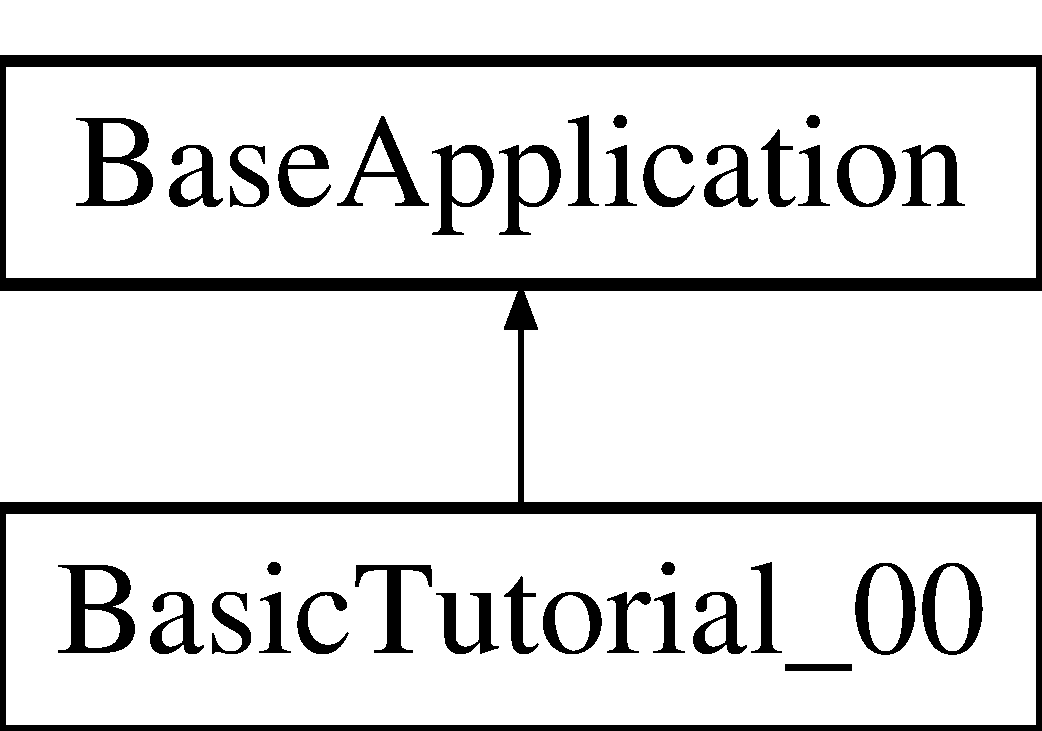
\includegraphics[height=2.000000cm]{class_base_application}
\end{center}
\end{figure}
\subsection*{Public Member Functions}
\begin{DoxyCompactItemize}
\item 
\hypertarget{class_base_application_a8a14a65a29118dd75173aa68678a05e1}{
virtual void {\bfseries go} (void)}
\label{class_base_application_a8a14a65a29118dd75173aa68678a05e1}

\end{DoxyCompactItemize}
\subsection*{Protected Member Functions}
\begin{DoxyCompactItemize}
\item 
\hypertarget{class_base_application_a5853d0e148cb85b0297a6885e1d33a89}{
virtual bool {\bfseries setup} ()}
\label{class_base_application_a5853d0e148cb85b0297a6885e1d33a89}

\item 
\hypertarget{class_base_application_a62ed46f90e9f82cc810997647a2c587e}{
virtual bool {\bfseries configure} (void)}
\label{class_base_application_a62ed46f90e9f82cc810997647a2c587e}

\item 
\hypertarget{class_base_application_ad5bc9655041e1849a4c13f444a3712bd}{
virtual void {\bfseries chooseSceneManager} (void)}
\label{class_base_application_ad5bc9655041e1849a4c13f444a3712bd}

\item 
\hypertarget{class_base_application_afa9d51527763cf9aee9cd4e1b1039d55}{
virtual void {\bfseries createCamera} (void)}
\label{class_base_application_afa9d51527763cf9aee9cd4e1b1039d55}

\item 
\hypertarget{class_base_application_aff6fd9ff1ff0978cc68f19dd65be4778}{
virtual void {\bfseries createFrameListener} (void)}
\label{class_base_application_aff6fd9ff1ff0978cc68f19dd65be4778}

\item 
\hypertarget{class_base_application_aa97beeb4059b17d0ec22eae33286ec2d}{
virtual void {\bfseries createScene} (void)=0}
\label{class_base_application_aa97beeb4059b17d0ec22eae33286ec2d}

\item 
\hypertarget{class_base_application_a365146059b25391fe400f5fdb94f011e}{
virtual void {\bfseries destroyScene} (void)}
\label{class_base_application_a365146059b25391fe400f5fdb94f011e}

\item 
\hypertarget{class_base_application_a1f8f6730cae6ec769d8730b1af48486e}{
virtual void {\bfseries createViewports} (void)}
\label{class_base_application_a1f8f6730cae6ec769d8730b1af48486e}

\item 
\hypertarget{class_base_application_ae27301702f1e5de64619a39b1929f1f9}{
virtual void {\bfseries setupResources} (void)}
\label{class_base_application_ae27301702f1e5de64619a39b1929f1f9}

\item 
\hypertarget{class_base_application_a9b77972f0f747a61e1f8ceba2ad47641}{
virtual void {\bfseries createResourceListener} (void)}
\label{class_base_application_a9b77972f0f747a61e1f8ceba2ad47641}

\item 
\hypertarget{class_base_application_aaeb764e637dd87601a81a80156659d88}{
virtual void {\bfseries loadResources} (void)}
\label{class_base_application_aaeb764e637dd87601a81a80156659d88}

\item 
\hypertarget{class_base_application_a03912a0f38b38fede7f08a2571e8fc56}{
virtual bool {\bfseries frameRenderingQueued} (const Ogre::FrameEvent \&evt)}
\label{class_base_application_a03912a0f38b38fede7f08a2571e8fc56}

\item 
\hypertarget{class_base_application_acfa977f04e435f18018ece805c1277ec}{
virtual bool {\bfseries keyPressed} (const OIS::KeyEvent \&arg)}
\label{class_base_application_acfa977f04e435f18018ece805c1277ec}

\item 
\hypertarget{class_base_application_aba5c7c9dea7a0efc58b89310bae547e5}{
virtual bool {\bfseries keyReleased} (const OIS::KeyEvent \&arg)}
\label{class_base_application_aba5c7c9dea7a0efc58b89310bae547e5}

\item 
\hypertarget{class_base_application_a126e59cb246b061e51eb6ce06a2ee8f4}{
virtual bool {\bfseries mouseMoved} (const OIS::MouseEvent \&arg)}
\label{class_base_application_a126e59cb246b061e51eb6ce06a2ee8f4}

\item 
\hypertarget{class_base_application_a9255dfc1eabefd11c474ec45a6622504}{
virtual bool {\bfseries mousePressed} (const OIS::MouseEvent \&arg, OIS::MouseButtonID id)}
\label{class_base_application_a9255dfc1eabefd11c474ec45a6622504}

\item 
\hypertarget{class_base_application_aa102c5859c14c0690c749994a446b53d}{
virtual bool {\bfseries mouseReleased} (const OIS::MouseEvent \&arg, OIS::MouseButtonID id)}
\label{class_base_application_aa102c5859c14c0690c749994a446b53d}

\item 
\hypertarget{class_base_application_afacf8a797588592ef0abbad593f10cfa}{
virtual void {\bfseries windowResized} (Ogre::RenderWindow $\ast$rw)}
\label{class_base_application_afacf8a797588592ef0abbad593f10cfa}

\item 
\hypertarget{class_base_application_ae0e37ac54a31ff6e51d58c7654ad1b90}{
virtual void {\bfseries windowClosed} (Ogre::RenderWindow $\ast$rw)}
\label{class_base_application_ae0e37ac54a31ff6e51d58c7654ad1b90}

\end{DoxyCompactItemize}
\subsection*{Protected Attributes}
\begin{DoxyCompactItemize}
\item 
\hypertarget{class_base_application_add84ba707dc6c57e6283f214b1274110}{
Ogre::Root $\ast$ {\bfseries mRoot}}
\label{class_base_application_add84ba707dc6c57e6283f214b1274110}

\item 
\hypertarget{class_base_application_a3829c6b12afe911e97e6b4524b33a38b}{
Ogre::Camera $\ast$ {\bfseries mCamera}}
\label{class_base_application_a3829c6b12afe911e97e6b4524b33a38b}

\item 
\hypertarget{class_base_application_a8a7684f4f9a57ed3089048ad1a913b2d}{
Ogre::SceneManager $\ast$ {\bfseries mSceneMgr}}
\label{class_base_application_a8a7684f4f9a57ed3089048ad1a913b2d}

\item 
\hypertarget{class_base_application_ac5d8e9c81e036897bc82f81eff8c570f}{
Ogre::RenderWindow $\ast$ {\bfseries mWindow}}
\label{class_base_application_ac5d8e9c81e036897bc82f81eff8c570f}

\item 
\hypertarget{class_base_application_a765e0df01c141a16df3178ab4f17afe6}{
Ogre::String {\bfseries mResourcesCfg}}
\label{class_base_application_a765e0df01c141a16df3178ab4f17afe6}

\item 
\hypertarget{class_base_application_a04f2fe47fa164fd78d986dc0df70b7fb}{
Ogre::String {\bfseries mPluginsCfg}}
\label{class_base_application_a04f2fe47fa164fd78d986dc0df70b7fb}

\item 
\hypertarget{class_base_application_a7faa397f4f4861ee8c361a01e90b4416}{
OgreBites::SdkTrayManager $\ast$ {\bfseries mTrayMgr}}
\label{class_base_application_a7faa397f4f4861ee8c361a01e90b4416}

\item 
\hypertarget{class_base_application_a9ae38dea6316058549151fff66a91fcd}{
OgreBites::SdkCameraMan $\ast$ {\bfseries mCameraMan}}
\label{class_base_application_a9ae38dea6316058549151fff66a91fcd}

\item 
\hypertarget{class_base_application_a6a11054ca61efdf558e0ff1b2de43a12}{
OgreBites::ParamsPanel $\ast$ {\bfseries mDetailsPanel}}
\label{class_base_application_a6a11054ca61efdf558e0ff1b2de43a12}

\item 
\hypertarget{class_base_application_ac7e861799862cb645f1d78b170aef80d}{
bool {\bfseries mCursorWasVisible}}
\label{class_base_application_ac7e861799862cb645f1d78b170aef80d}

\item 
\hypertarget{class_base_application_a755f26d3a9915aaf830750d877e39d86}{
bool {\bfseries mShutDown}}
\label{class_base_application_a755f26d3a9915aaf830750d877e39d86}

\item 
\hypertarget{class_base_application_abc9503c8462e225b5d0d55c952d9e4a9}{
OIS::InputManager $\ast$ {\bfseries mInputManager}}
\label{class_base_application_abc9503c8462e225b5d0d55c952d9e4a9}

\item 
\hypertarget{class_base_application_add9b97fbe64da2814d3af113bac58c43}{
OIS::Mouse $\ast$ {\bfseries mMouse}}
\label{class_base_application_add9b97fbe64da2814d3af113bac58c43}

\item 
\hypertarget{class_base_application_a9d6e19cf50c47379fbaae55bff28079c}{
OIS::Keyboard $\ast$ {\bfseries mKeyboard}}
\label{class_base_application_a9d6e19cf50c47379fbaae55bff28079c}

\end{DoxyCompactItemize}


The documentation for this class was generated from the following files:\begin{DoxyCompactItemize}
\item 
D:/wingo/teaching\_\-course\_\-2011/3DGameProgramming/source\_\-code/3DGame\_\-Ogre\_\-vc\_\-9\_\-v1-\/7-\/1\_\-Assigns/programs\_\-beginner/Assign\_\-01\_\-MultiViewports/source/BaseApplication.h\item 
D:/wingo/teaching\_\-course\_\-2011/3DGameProgramming/source\_\-code/3DGame\_\-Ogre\_\-vc\_\-9\_\-v1-\/7-\/1\_\-Assigns/programs\_\-beginner/Assign\_\-01\_\-MultiViewports/source/BaseApplication.cpp\end{DoxyCompactItemize}

\hypertarget{class_basic_tutorial__00}{
\section{BasicTutorial\_\-00 Class Reference}
\label{class_basic_tutorial__00}\index{BasicTutorial\_\-00@{BasicTutorial\_\-00}}
}


3D Game Programming \par
 My Name: AA BB CC \par
 My ID: 0123456789 \par
 My Email: \href{mailto:aaa@cs.nctu.edu.tw}{\tt aaa@cs.nctu.edu.tw}  




{\ttfamily \#include $<$TutorialApplication.h$>$}

Inheritance diagram for BasicTutorial\_\-00:\begin{figure}[H]
\begin{center}
\leavevmode
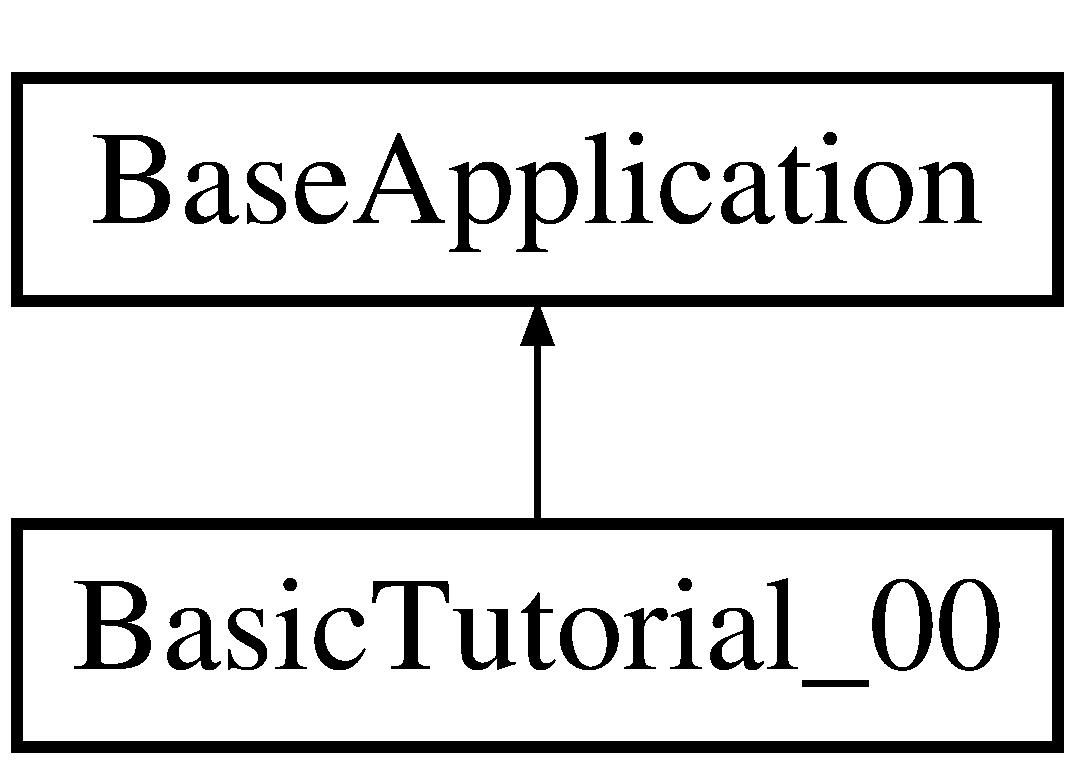
\includegraphics[height=2.000000cm]{class_basic_tutorial__00}
\end{center}
\end{figure}
\subsection*{Public Member Functions}
\begin{DoxyCompactItemize}
\item 
\hypertarget{class_basic_tutorial__00_adc2454d9f8226e0958ecf702f355846e}{
virtual void {\bfseries createViewports} (void)}
\label{class_basic_tutorial__00_adc2454d9f8226e0958ecf702f355846e}

\item 
\hypertarget{class_basic_tutorial__00_a15a3d4673724ec99077ce992f996a550}{
virtual void {\bfseries createScene} (void)}
\label{class_basic_tutorial__00_a15a3d4673724ec99077ce992f996a550}

\item 
\hypertarget{class_basic_tutorial__00_a1bf709417d654dffc2ea10987412b912}{
virtual void {\bfseries createCamera} (void)}
\label{class_basic_tutorial__00_a1bf709417d654dffc2ea10987412b912}

\item 
\hypertarget{class_basic_tutorial__00_aba97a29d983586d2dc8e108d3bccf721}{
virtual void {\bfseries chooseSceneManager} (void)}
\label{class_basic_tutorial__00_aba97a29d983586d2dc8e108d3bccf721}

\end{DoxyCompactItemize}


\subsection{Detailed Description}
3D Game Programming \par
 My Name: AA BB CC \par
 My ID: 0123456789 \par
 My Email: \href{mailto:aaa@cs.nctu.edu.tw}{\tt aaa@cs.nctu.edu.tw} This is an assignment of 3D Game Programming 

The documentation for this class was generated from the following files:\begin{DoxyCompactItemize}
\item 
D:/wingo/teaching\_\-course\_\-2011/3DGameProgramming/source\_\-code/3DGame\_\-Ogre\_\-vc\_\-9\_\-v1-\/7-\/1\_\-Assigns/programs\_\-beginner/Assign\_\-01\_\-MultiViewports/source/TutorialApplication.h\item 
D:/wingo/teaching\_\-course\_\-2011/3DGameProgramming/source\_\-code/3DGame\_\-Ogre\_\-vc\_\-9\_\-v1-\/7-\/1\_\-Assigns/programs\_\-beginner/Assign\_\-01\_\-MultiViewports/source/TutorialApplication.cpp\end{DoxyCompactItemize}

\printindex
\end{document}
